\documentclass[11pt,a4paper]{article}
\usepackage[top=2cm, bottom=2.3cm, left=1.8cm, right=1.8cm, headsep=0.8cm]{geometry}
\usepackage{amsmath,amssymb,amsfonts}
\usepackage{graphicx}
\graphicspath{{images/}{public/exam-images/SohanMock/}{./}}
\usepackage{enumitem}
\usepackage{fancyhdr}
\usepackage[table]{xcolor}
\usepackage{tcolorbox}
\tcbuselibrary{breakable,skins}
\usepackage{tabularx}
\usepackage{multicol}

% High-Contrast Modern Color Palette
\definecolor{primaryDark}{RGB}{12, 32, 84}       % Midnight Navy (Deep)
\definecolor{primaryBlue}{RGB}{18, 72, 160}      % Solid Royal Blue
\definecolor{goldAccent}{RGB}{255, 215, 0}       % Gold highlight
\definecolor{l1Green}{RGB}{14, 120, 62}          % Vivid Forest Green
\definecolor{l2Amber}{RGB}{205, 80, 0}           % Rich Amber / Orange
\definecolor{l3Crimson}{RGB}{180, 20, 20}        % Deep Crimson Red
\definecolor{formulaBg}{RGB}{255, 252, 235}      % Warm Cream-Gold
\definecolor{formulaBorder}{RGB}{220, 160, 30}   % Gold Border
\definecolor{cardBg}{RGB}{250, 252, 255}         % Clean Crisp Card Background
\definecolor{cardBorder}{RGB}{130, 170, 220}     % Sharp Steel Blue Border
\definecolor{tableStripe}{RGB}{242, 246, 252}    % Alternating Table Row
\definecolor{tableDarkHeader}{RGB}{12, 32, 84}   % Dark Table Header
\definecolor{darkCharcoal}{RGB}{25, 25, 25}      % High-contrast body text

% Page styling
\pagestyle{fancy}
\fancyhf{}
\setlength{\headheight}{16pt}
\fancyhead[L]{\small\textsf{\textbf{\textcolor{primaryDark}{Sohan Mocks Series}} $\vert$ \textbf{\textcolor{primaryBlue}{Physics: Gravitation (JEE Main Medium)}}}}
\fancyhead[R]{\small\textsf{\textbf{\textcolor{l1Green}{Max Marks: 100 $\vert$ 60 Mins}}}}
\fancyfoot[C]{\textbf{\textsf{\thepage}}}
\renewcommand{\headrulewidth}{0.8pt}
\renewcommand{\footrulewidth}{0.4pt}

% Custom High-Contrast tcolorboxes
\tcbset{
  dayheader/.style={
    colback=primaryDark,
    coltext=white,
    boxrule=0pt,
    arc=3mm,
    left=14pt, right=14pt, top=10pt, bottom=10pt
  },
  sectionbanner/.style={
    colback=primaryBlue,
    coltext=white,
    boxrule=0pt,
    arc=2mm,
    left=10pt, right=10pt, top=6pt, bottom=6pt
  },
  solbox/.style={
    enhanced,
    breakable,
    colback=cardBg,
    colframe=cardBorder,
    boxrule=1.0pt,
    arc=2mm,
    left=10pt, right=10pt, top=7pt, bottom=7pt
  }
}

\begin{document}

% ==================== TEST HEADER BANNER ====================
\begin{tcolorbox}[dayheader]
\begin{center}
  {\Large \textbf{\textsf{\textcolor{goldAccent}{SOHAN MOCKS TEST SERIES}}}}\\[3pt]
  {\LARGE \textbf{\textsf{TOPICAL SPECIAL: GRAVITATION (JEE MAIN MEDIUM PAPER)}}}\\[5pt]
  {\normalsize \textbf{\textsf{Core Domains:}} Variation of $g$ $\vert$ Escape Speed $\vert$ Kepler's Laws $\vert$ Satellite Energy $\vert$ Neutral Points $\vert$ Earth Tunnels}\\[3pt]
  {\footnotesize \textbf{Exam Pattern:} 25 Questions (20 MCQs $+4/-1$ + 5 Numerical $+4/0$) \quad $\vert$ \quad \textbf{Time:} 60 Minutes \quad $\vert$ \quad \textbf{Max Marks:} 100}
\end{center}
\end{tcolorbox}

\vspace{6pt}

% ==================== SECTION I: SINGLE CORRECT CHOICE ====================
\begin{tcolorbox}[sectionbanner]
  {\large \textbf{\textsf{SECTION I: SINGLE CORRECT CHOICE TYPE (Q01 -- Q20)}}} \hfill {\small \textbf{Marking: $+4$ / $-1$}}
\end{tcolorbox}
\vspace{4pt}

\begin{enumerate}[label=\textbf{\arabic*.},leftmargin=18pt,itemsep=10pt]

  \item At what height $h$ above the surface of Earth (radius $R$) does the acceleration due to gravity reduce to $\dfrac{1}{9}\text{th}$ of its value on the surface?
  \begin{multicols}{4}
    \begin{enumerate}[label=(\Alph*)]
      \item $R$
      \item $2R$
      \item $3R$
      \item $8R$
    \end{enumerate}
  \end{multicols}

  \item A body has a weight of $250\text{ N}$ on the surface of the Earth. How much will it weigh halfway down to the center of the Earth?
  \begin{multicols}{2}
    \begin{enumerate}[label=(\Alph*)]
      \item $125\text{ N}$
      \item $150\text{ N}$
      \item $62.5\text{ N}$
      \item $200\text{ N}$
    \end{enumerate}
  \end{multicols}

  \item The value of acceleration due to gravity at a small height $h = 5\text{ km}$ above Earth's surface is equal to its value at a depth $d$ below Earth's surface. Assuming $h \ll R$, the depth $d$ is:
  \begin{multicols}{2}
    \begin{enumerate}[label=(\Alph*)]
      \item $2.5\text{ km}$
      \item $5\text{ km}$
      \item $10\text{ km}$
      \item $20\text{ km}$
    \end{enumerate}
  \end{multicols}

  \item The distance between the centers of the Earth (mass $M$) and the Moon (mass $m = \dfrac{M}{81}$) is $D$, as illustrated in the figure. At what distance $x$ from the center of the Earth along the line joining their centers is the net gravitational field intensity strictly zero?
  \begin{center}
    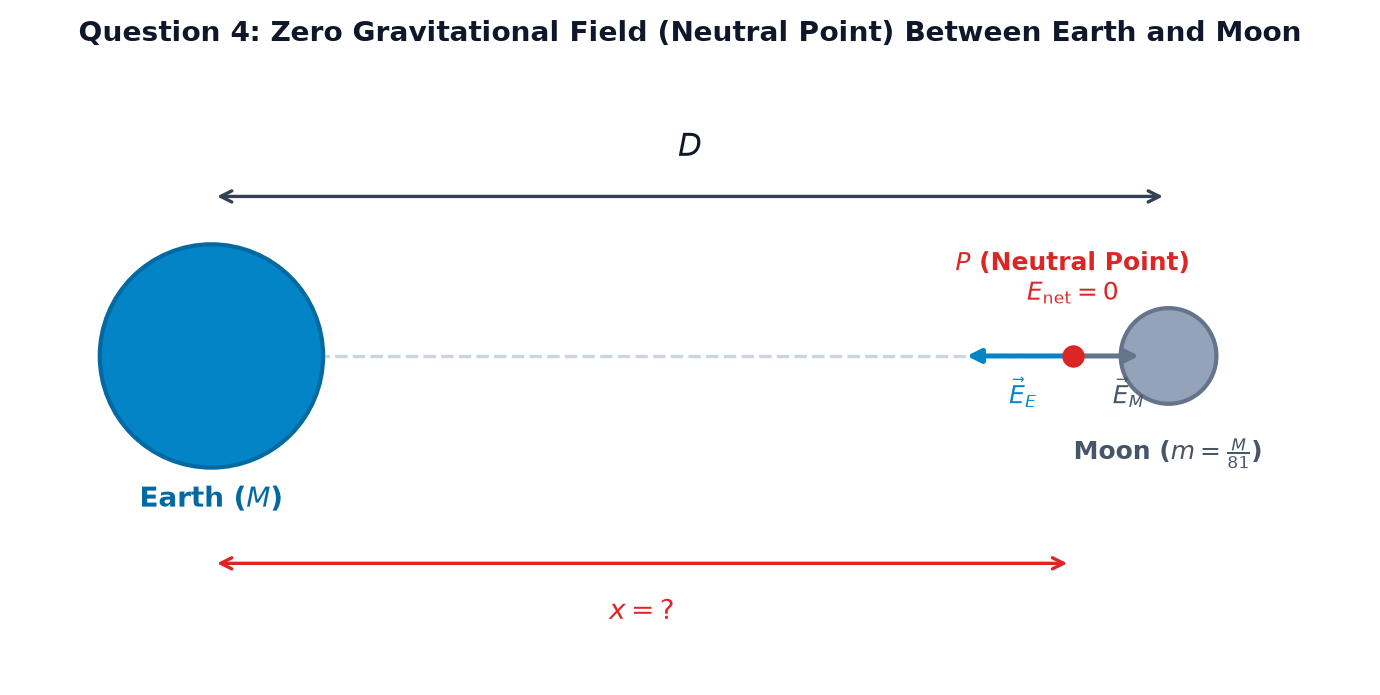
\includegraphics[width=0.42\textwidth]{images/sohan_grav_med_q04_neutral.png}
  \end{center}
  \begin{multicols}{2}
    \begin{enumerate}[label=(\Alph*)]
      \item $\dfrac{9}{10}D$
      \item $\dfrac{8}{9}D$
      \item $\dfrac{1}{10}D$
      \item $\dfrac{1}{9}D$
    \end{enumerate}
  \end{multicols}

  \item The escape velocity of a body from Earth's surface is $v_e = 11.2\text{ km/s}$. A newly discovered planet has mass equal to $8$ times Earth's mass and radius equal to $2$ times Earth's radius. The escape velocity from the surface of this planet is:
  \begin{multicols}{2}
    \begin{enumerate}[label=(\Alph*)]
      \item $11.2\text{ km/s}$
      \item $22.4\text{ km/s}$
      \item $44.8\text{ km/s}$
      \item $5.6\text{ km/s}$
    \end{enumerate}
  \end{multicols}

  \item A satellite of mass $m$ is moving in a circular orbit of radius $r$ around Earth (mass $M$). The ratio of its kinetic energy $K$ to its gravitational potential energy $U$ is:
  \begin{multicols}{2}
    \begin{enumerate}[label=(\Alph*)]
      \item $-\dfrac{1}{2}$
      \item $\dfrac{1}{2}$
      \item $-2$
      \item $-1$
    \end{enumerate}
  \end{multicols}

  \item Two satellites $A$ and $B$ are orbiting Earth in circular orbits of radii $R_0$ and $4R_0$ respectively. If the orbital period of satellite $A$ is $8\text{ days}$, the orbital period of satellite $B$ is:
  \begin{multicols}{2}
    \begin{enumerate}[label=(\Alph*)]
      \item $16\text{ days}$
      \item $32\text{ days}$
      \item $64\text{ days}$
      \item $128\text{ days}$
    \end{enumerate}
  \end{multicols}

  \item For a uniform solid sphere of mass $M$ and radius $R$, the gravitational potential $V(r)$ varies with radial distance $r$ from the center as shown in the graph. What are the values of gravitational potential at the center ($r = 0$) and at the surface ($r = R$)?
  \begin{center}
    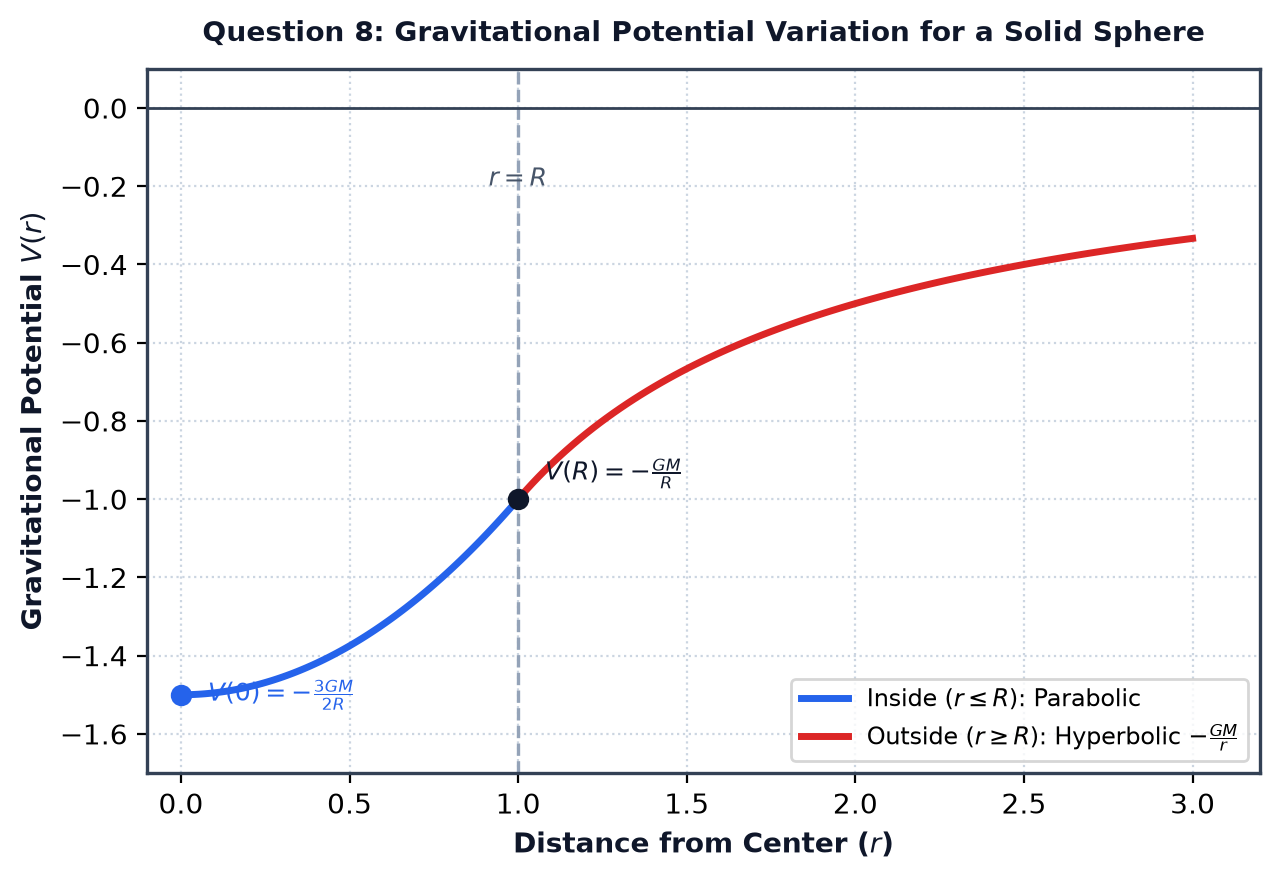
\includegraphics[width=0.38\textwidth]{images/sohan_grav_med_q08_potential_graph.png}
  \end{center}
  \begin{enumerate}[label=(\Alph*)]
    \item $V(0) = -\dfrac{GM}{R}, \quad V(R) = -\dfrac{GM}{2R}$
    \item $V(0) = -\dfrac{3GM}{2R}, \quad V(R) = -\dfrac{GM}{R}$
    \item $V(0) = 0, \quad V(R) = -\dfrac{GM}{R}$
    \item $V(0) = -\dfrac{2GM}{R}, \quad V(R) = -\dfrac{GM}{R}$
  \end{enumerate}

  \item The amount of work done by an external agent to slowly lift a body of mass $m$ from the surface of Earth (radius $R$, surface gravity $g$) to a height $h = R$ above the surface is:
  \begin{multicols}{2}
    \begin{enumerate}[label=(\Alph*)]
      \item $mgR$
      \item $\dfrac{1}{2}mgR$
      \item $2mgR$
      \item $\dfrac{1}{4}mgR$
    \end{enumerate}
  \end{multicols}

  \item The apparent acceleration due to gravity at latitude $\lambda$ on Earth of radius $R$ is $g' = g - \omega^2 R \cos^2\lambda$. If the Earth speeds up its rotation so that bodies on the equator experience weightlessness ($g' = 0$), the angular velocity $\omega$ of the Earth must become:
  \begin{multicols}{2}
    \begin{enumerate}[label=(\Alph*)]
      \item $\sqrt{\dfrac{g}{R}}$
      \item $\sqrt{\dfrac{2g}{R}}$
      \item $\sqrt{\dfrac{g}{2R}}$
      \item $\dfrac{g}{R}$
    \end{enumerate}
  \end{multicols}

  \item Which of the following statements regarding a geostationary satellite is INCORRECT?
  \begin{enumerate}[label=(\Alph*)]
    \item Its orbital period is 24 hours
    \item Its sense of rotation is from West to East
    \item It can be placed in an orbit at any arbitrary latitude as long as its altitude is approximately $36,000\text{ km}$
    \item Its orbital plane must strictly coincide with the equatorial plane of the Earth
  \end{enumerate}

  \item A binary star system consists of two stars of masses $m_1 = 2M$ and $m_2 = M$ separated by a distance $r$. They move in concentric circular orbits around their common center of mass under their mutual gravitational attraction, as shown in the figure. The ratio of their orbital radii $\dfrac{r_1}{r_2}$ and the ratio of their orbital speeds $\dfrac{v_1}{v_2}$ are:
  \begin{center}
    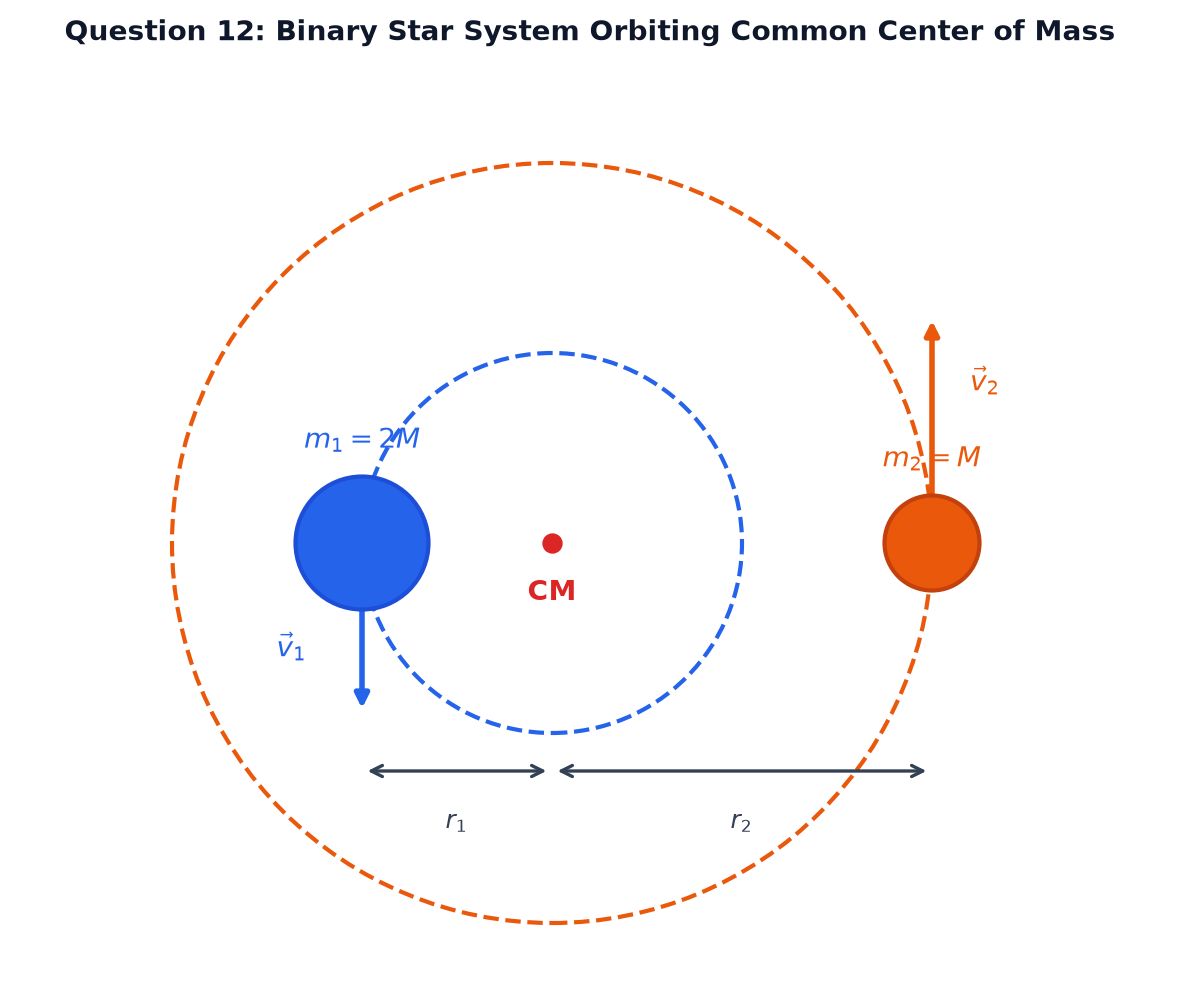
\includegraphics[width=0.36\textwidth]{images/sohan_grav_med_q12_binary_star.png}
  \end{center}
  \begin{enumerate}[label=(\Alph*)]
    \item $\dfrac{r_1}{r_2} = \dfrac{1}{2}, \quad \dfrac{v_1}{v_2} = \dfrac{1}{2}$
    \item $\dfrac{r_1}{r_2} = 2, \quad \dfrac{v_1}{v_2} = 2$
    \item $\dfrac{r_1}{r_2} = \dfrac{1}{2}, \quad \dfrac{v_1}{v_2} = 1$
    \item $\dfrac{r_1}{r_2} = \dfrac{1}{4}, \quad \dfrac{v_1}{v_2} = \dfrac{1}{2}$
  \end{enumerate}

  \item A thin uniform spherical shell has mass $M$ and radius $R$. A point mass $m$ is placed inside the shell at a distance $r = \dfrac{R}{2}$ from its center. The gravitational force exerted by the shell on the point mass is:
  \begin{multicols}{2}
    \begin{enumerate}[label=(\Alph*)]
      \item $\text{Zero}$
      \item $\dfrac{GMm}{R^2}$
      \item $\dfrac{2GMm}{R^2}$
      \item $\dfrac{4GMm}{R^2}$
    \end{enumerate}
  \end{multicols}

  \item A satellite is moving in a circular orbit grazing Earth's surface with orbital speed $v_o$. What is the minimum percentage increase in its speed required for it to escape Earth's gravitational field completely?
  \begin{multicols}{4}
    \begin{enumerate}[label=(\Alph*)]
      \item $41.4\%$
      \item $50.0\%$
      \item $100\%$
      \item $20.7\%$
    \end{enumerate}
  \end{multicols}

  \item Four identical particles, each of mass $m$, are placed at the vertices of a square of side $a$, as illustrated in the figure. The work done by an external agent to assemble this system from an initial state where all particles were infinitely separated is:
  \begin{center}
    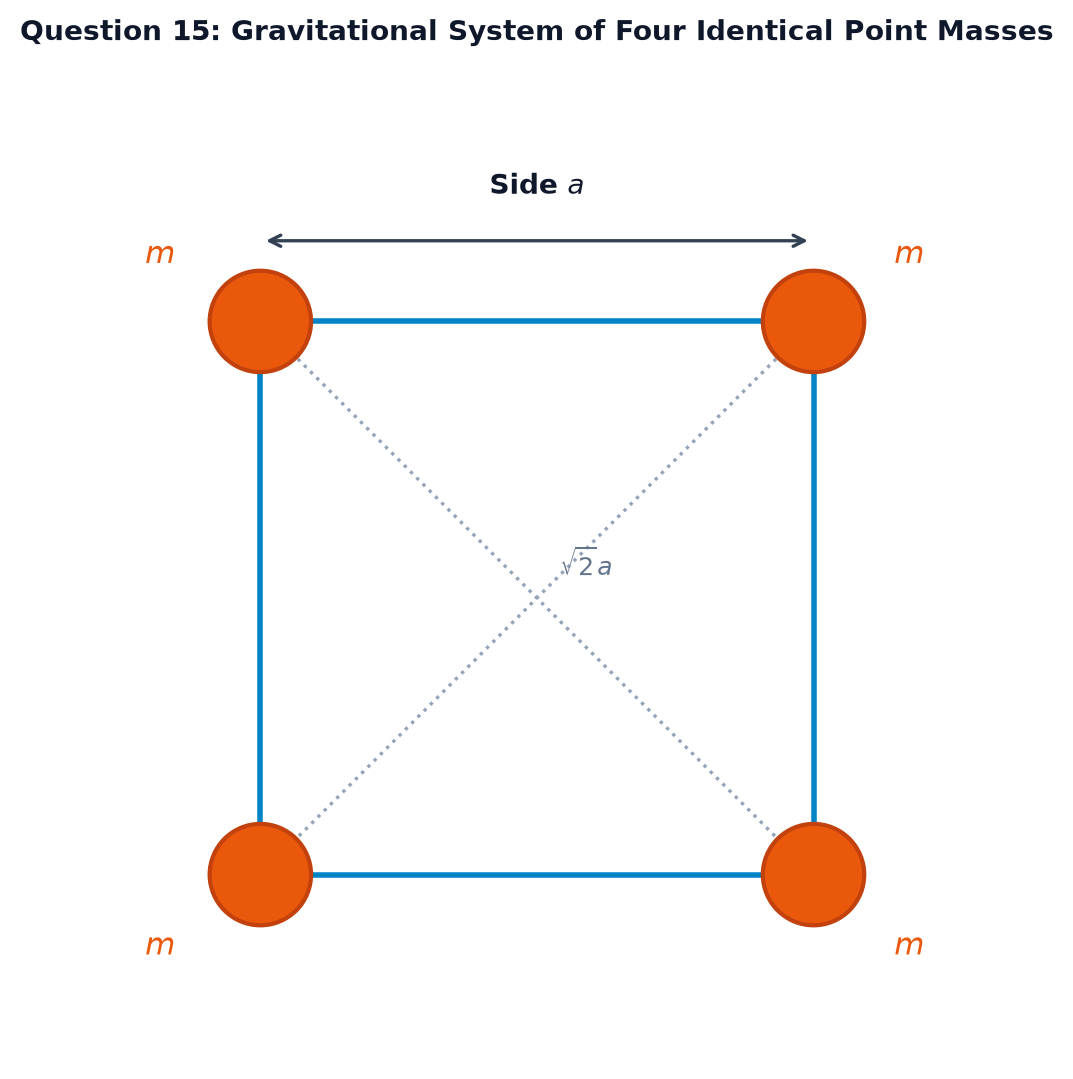
\includegraphics[width=0.34\textwidth]{images/sohan_grav_med_q15_square_particles.png}
  \end{center}
  \begin{multicols}{2}
    \begin{enumerate}[label=(\Alph*)]
      \item $-(4 + \sqrt{2})\dfrac{Gm^2}{a}$
      \item $-(4 + 2\sqrt{2})\dfrac{Gm^2}{a}$
      \item $-\dfrac{6Gm^2}{a}$
      \item $-(2 + \sqrt{2})\dfrac{Gm^2}{a}$
    \end{enumerate}
  \end{multicols}

  \item A body is projected vertically upwards from the surface of Earth with a speed equal to $\dfrac{1}{2}$ of the escape velocity ($v = \dfrac{v_e}{2}$). The maximum height $h$ reached by the body above the surface of the Earth is:
  \begin{multicols}{2}
    \begin{enumerate}[label=(\Alph*)]
      \item $\dfrac{R}{3}$
      \item $\dfrac{R}{2}$
      \item $\dfrac{R}{4}$
      \item $\dfrac{2R}{3}$
    \end{enumerate}
  \end{multicols}

  \item If the mean density $\rho$ of Earth were doubled while keeping its radius $R$ unchanged, what would happen to the surface acceleration due to gravity $g$ and the orbital period $T$ of a low-altitude satellite?
  \begin{enumerate}[label=(\Alph*)]
    \item $g$ doubles, $T$ becomes $\dfrac{T}{\sqrt{2}}$
    \item $g$ quadruples, $T$ halves
    \item $g$ halves, $T$ doubles
    \item $g$ doubles, $T$ remains unchanged
  \end{enumerate}

  \item A satellite of mass $m = 1000\text{ kg}$ is revolving in a circular orbit at an altitude equal to the Earth's radius ($h = R$) above Earth's surface. Taking $g = 10\text{ m/s}^2$ and Earth radius $R = 6.4 \times 10^6\text{ m}$, the binding energy of the satellite is:
  \begin{multicols}{2}
    \begin{enumerate}[label=(\Alph*)]
      \item $1.6 \times 10^{10}\text{ J}$
      \item $3.2 \times 10^{10}\text{ J}$
      \item $6.4 \times 10^{10}\text{ J}$
      \item $8.0 \times 10^{9}\text{ J}$
    \end{enumerate}
  \end{multicols}

  \item A smooth tunnel is bored through the center of the Earth along a diameter, as depicted in the figure. A particle of mass $m$ is released from rest inside the tunnel at a radial distance $r$ from the center ($r \le R$). Which of the following expressions correctly gives the gravitational restoring force $F(r)$ acting on the particle?
  \begin{center}
    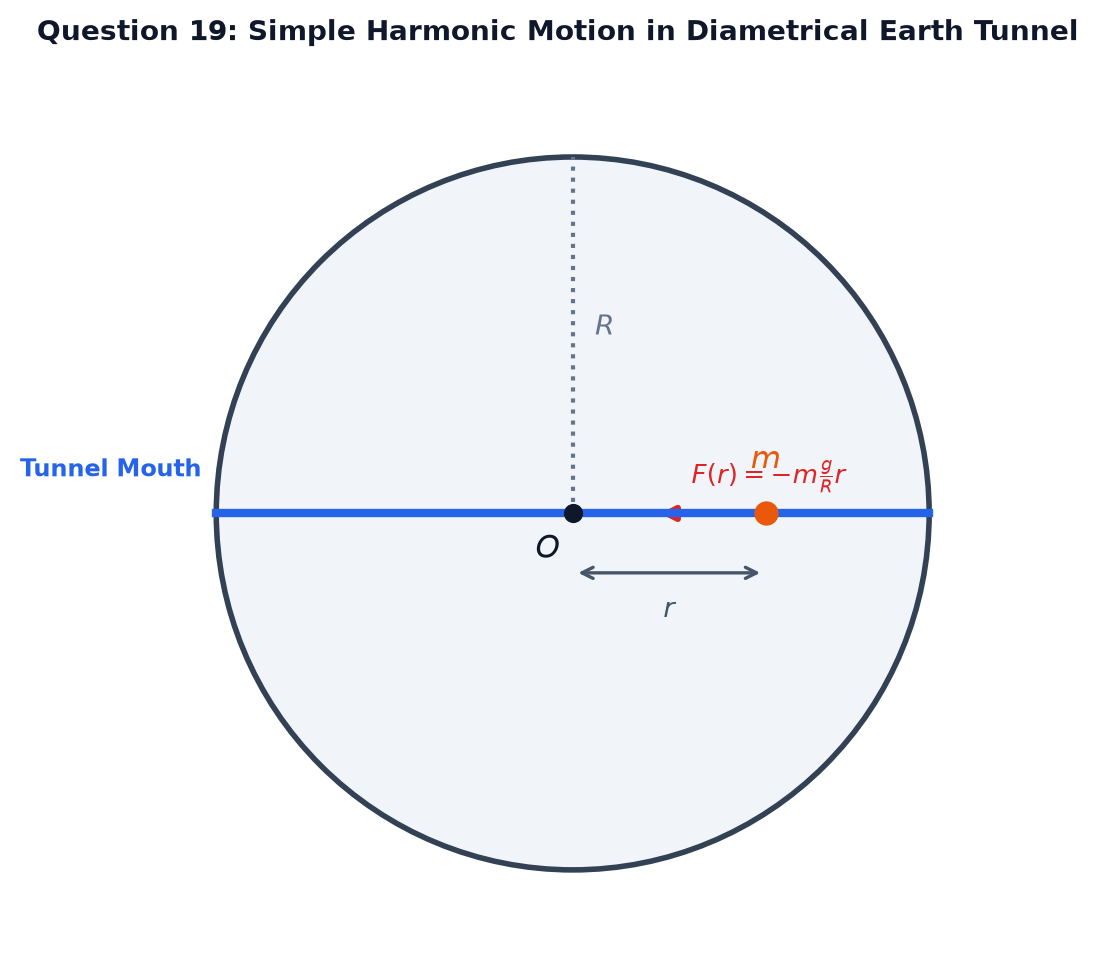
\includegraphics[width=0.36\textwidth]{images/sohan_grav_med_q19_tunnel_shm.png}
  \end{center}
  \begin{multicols}{2}
    \begin{enumerate}[label=(\Alph*)]
      \item $F(r) = -m \dfrac{g}{R^2} r^2$
      \item $F(r) = -m \dfrac{g}{R} r$
      \item $F(r) = -m \dfrac{g R^2}{r^2}$
      \item $F(r) = -m g$
    \end{enumerate}
  \end{multicols}

  \item The Moon lacks an atmosphere primarily because:
  \begin{enumerate}[label=(\Alph*)]
    \item The root mean square speed ($v_{\text{rms}}$) of atmospheric gas molecules exceeds the escape velocity on the Moon's surface
    \item The surface temperature on the Moon is too low for gases to exist
    \item The gravitational attraction of the Sun pulls the gases away from the Moon
    \item The Moon does not rotate on its axis
  \end{enumerate}

\end{enumerate}

\vspace{10pt}

% ==================== SECTION II: NUMERICAL VALUE TYPE ====================
\begin{tcolorbox}[sectionbanner]
  {\large \textbf{\textsf{SECTION II: NUMERICAL VALUE TYPE (Q21 -- Q25)}}} \hfill {\small \textbf{Marking: $+4$ / $0$}}
\end{tcolorbox}
\vspace{4pt}

\begin{enumerate}[label=\textbf{\arabic*.},leftmargin=18pt,itemsep=12pt,resume]

  \item A communication satellite is in a circular orbit of radius $r_1$ with an orbital period of $24\text{ hours}$. Another satellite in circular orbit around the same planet has an orbital period of $3\text{ hours}$. If the radius of its orbit is $\dfrac{r_1}{N}$, find the integer value of $N$.

  \item The acceleration due to gravity at a height $h = k R$ above Earth's surface becomes $25\%$ of its value on the surface (where $R$ is the radius of the Earth). Find the integer value of $k$.

  \item A total mass $M$ is split into two parts of masses $m_1 = x M$ and $m_2 = (1 - x)M$. When placed at a fixed distance $r$, the gravitational force of attraction between them is maximum when $x = \dfrac{1}{k}$. Find the integer value of $k$.

  \item A particle is dropped from the surface of Earth into a smooth diametrical tunnel bored through Earth's center. The particle undergoes simple harmonic motion with time period $T$. If the time taken by the particle to travel from the surface to the center of Earth is $t = \dfrac{T}{N}$, find the integer value of $N$.

  \item Two fixed spherical masses $M$ and $16M$ have their centers separated by a distance $D = 100\text{ km}$ in deep space. A point along the line of centers between them where the net gravitational field is zero is located at a distance $d = k\text{ km}$ from the smaller mass $M$. Find the integer value of $k$.

\end{enumerate}

\newpage

% ==================== MASTER ANSWER KEY ====================
\begin{tcolorbox}[sectionbanner]
  {\large \textbf{\textsf{MASTER 100\% VERIFIED ANSWER KEY}}}
\end{tcolorbox}
\vspace{4pt}

\begin{center}
\renewcommand{\arraystretch}{1.25}
\small
\begin{tabularx}{\textwidth}{|>{\centering\arraybackslash}c|>{\centering\arraybackslash}c|>{\centering\arraybackslash}c|>{\centering\arraybackslash}c|>{\centering\arraybackslash}c|>{\centering\arraybackslash}c|>{\centering\arraybackslash}c|>{\centering\arraybackslash}c|>{\centering\arraybackslash}c|>{\centering\arraybackslash}X|}
\hline
\rowcolor{tableDarkHeader}
\textcolor{white}{\textbf{Q.}} & \textcolor{white}{\textbf{Ans}} & \textcolor{white}{\textbf{Q.}} & \textcolor{white}{\textbf{Ans}} & \textcolor{white}{\textbf{Q.}} & \textcolor{white}{\textbf{Ans}} & \textcolor{white}{\textbf{Q.}} & \textcolor{white}{\textbf{Ans}} & \textcolor{white}{\textbf{Q.}} & \textcolor{white}{\textbf{Ans}} \\
\hline
\rowcolor{white}
\textbf{01} & B & \textbf{06} & A & \textbf{11} & C & \textbf{16} & A & \textbf{21} & \textbf{4} \\
\hline
\rowcolor{tableStripe}
\textbf{02} & A & \textbf{07} & C & \textbf{12} & A & \textbf{17} & A & \textbf{22} & \textbf{1} \\
\hline
\rowcolor{white}
\textbf{03} & C & \textbf{08} & B & \textbf{13} & A & \textbf{18} & A & \textbf{23} & \textbf{2} \\
\hline
\rowcolor{tableStripe}
\textbf{04} & A & \textbf{09} & B & \textbf{14} & A & \textbf{19} & B & \textbf{24} & \textbf{4} \\
\hline
\rowcolor{white}
\textbf{05} & B & \textbf{10} & A & \textbf{15} & A & \textbf{20} & A & \textbf{25} & \textbf{20} \\
\hline
\end{tabularx}
\end{center}

\vspace{10pt}

% ==================== COMPREHENSIVE SOLUTIONS ====================
\begin{tcolorbox}[sectionbanner]
  {\large \textbf{\textsf{COMPREHENSIVE STEP-BY-STEP SOLUTIONS}}}
\end{tcolorbox}
\vspace{4pt}

\begin{tcolorbox}[solbox]
  \textbf{\textcolor{primaryDark}{Question 1:}} \hfill \textbf{\textcolor{l1Green}{Answer: B}}\\
  \vspace{3pt}
  The variation of acceleration due to gravity with height $h$ is given by:
$$g_h = \frac{g}{\left(1 + \dfrac{h}{R}\right)^2}$$
\vspace{3pt}
Given that $g_h = \dfrac{g}{9}$:
$$\frac{g}{\left(1 + \dfrac{h}{R}\right)^2} = \frac{g}{9} \implies 1 + \frac{h}{R} = 3 \implies \frac{h}{R} = 2 \implies h = 2R$$
\vspace{3pt}
Hence, the correct option is \textbf{(B)}.
\end{tcolorbox}
\vspace{3pt}

\begin{tcolorbox}[solbox]
  \textbf{\textcolor{primaryDark}{Question 2:}} \hfill \textbf{\textcolor{l1Green}{Answer: A}}\\
  \vspace{3pt}
  The acceleration due to gravity at depth $d$ below the Earth's surface is given by:
$$g_d = g\left(1 - \frac{d}{R}\right)$$
\vspace{3pt}
At halfway down to the center, the depth is $d = \dfrac{R}{2}$:
$$g_d = g\left(1 - \frac{R/2}{R}\right) = g\left(1 - \frac{1}{2}\right) = \frac{g}{2}$$
\vspace{3pt}
Therefore, the weight of the body at this depth is:
$$W' = m g_d = m \left(\frac{g}{2}\right) = \frac{W}{2} = \frac{250\text{ N}}{2} = 125\text{ N}$$
\vspace{3pt}
Hence, the correct option is \textbf{(A)}.
\end{tcolorbox}
\vspace{3pt}

\begin{tcolorbox}[solbox]
  \textbf{\textcolor{primaryDark}{Question 3:}} \hfill \textbf{\textcolor{l1Green}{Answer: C}}\\
  \vspace{3pt}
  For small heights $h \ll R$, the acceleration due to gravity is approximately:
$$g_h \approx g\left(1 - \frac{2h}{R}\right)$$
\vspace{3pt}
At depth $d$, the acceleration due to gravity is:
$$g_d = g\left(1 - \frac{d}{R}\right)$$
\vspace{3pt}
Equating $g_h = g_d$:
$$g\left(1 - \frac{2h}{R}\right) = g\left(1 - \frac{d}{R}\right) \implies \frac{2h}{R} = \frac{d}{R} \implies d = 2h$$
\vspace{3pt}
Given $h = 5\text{ km}$:
$$d = 2 \times 5\text{ km} = 10\text{ km}$$
\vspace{3pt}
Hence, the correct option is \textbf{(C)}.
\end{tcolorbox}
\vspace{3pt}

\begin{tcolorbox}[solbox]
  \textbf{\textcolor{primaryDark}{Question 4:}} \hfill \textbf{\textcolor{l1Green}{Answer: A}}\\
  \vspace{3pt}
  Let $P$ be the neutral point at distance $x$ from the Earth's center. Its distance from the Moon's center is $(D - x)$.
\vspace{3pt}
At point $P$, the gravitational field due to Earth balances that due to Moon:
$$\frac{GM}{x^2} = \frac{G(M/81)}{(D - x)^2}$$
\vspace{3pt}
Taking square roots on both sides:
$$\frac{1}{x} = \frac{1}{9(D - x)} \implies 9(D - x) = x \implies 9D - 9x = x \implies 10x = 9D \implies x = \frac{9}{10}D$$
\vspace{3pt}
Hence, the correct option is \textbf{(A)}.
\end{tcolorbox}
\vspace{3pt}

\begin{tcolorbox}[solbox]
  \textbf{\textcolor{primaryDark}{Question 5:}} \hfill \textbf{\textcolor{l1Green}{Answer: B}}\\
  \vspace{3pt}
  The escape velocity from a spherical body of mass $M$ and radius $R$ is:
$$v_e = \sqrt{\frac{2GM}{R}}$$
\vspace{3pt}
For the newly discovered planet with $M' = 8M$ and $R' = 2R$:
$$v_p = \sqrt{\frac{2G(8M)}{2R}} = \sqrt{4 \times \frac{2GM}{R}} = 2\sqrt{\frac{2GM}{R}} = 2 v_e$$
\vspace{3pt}
Given $v_e = 11.2\text{ km/s}$:
$$v_p = 2 \times 11.2\text{ km/s} = 22.4\text{ km/s}$$
\vspace{3pt}
Hence, the correct option is \textbf{(B)}.
\end{tcolorbox}
\vspace{3pt}

\begin{tcolorbox}[solbox]
  \textbf{\textcolor{primaryDark}{Question 6:}} \hfill \textbf{\textcolor{l1Green}{Answer: A}}\\
  \vspace{3pt}
  For a satellite in circular orbit of radius $r$, centripetal force is provided by gravity:
$$\frac{m v^2}{r} = \frac{GMm}{r^2} \implies m v^2 = \frac{GMm}{r}$$
\vspace{3pt}
Kinetic energy:
$$K = \frac{1}{2}m v^2 = \frac{GMm}{2r}$$
\vspace{3pt}
Gravitational potential energy:
$$U = -\frac{GMm}{r}$$
\vspace{3pt}
Taking their ratio:
$$\frac{K}{U} = \frac{\dfrac{GMm}{2r}}{-\dfrac{GMm}{r}} = -\frac{1}{2}$$
\vspace{3pt}
Hence, the correct option is \textbf{(A)}.
\end{tcolorbox}
\vspace{3pt}

\begin{tcolorbox}[solbox]
  \textbf{\textcolor{primaryDark}{Question 7:}} \hfill \textbf{\textcolor{l1Green}{Answer: C}}\\
  \vspace{3pt}
  According to Kepler's Third Law of planetary motion:
$$T^2 \propto r^3 \implies \frac{T_B}{T_A} = \left(\frac{r_B}{r_A}\right)^{3/2}$$
\vspace{3pt}
Given $r_A = R_0$ and $r_B = 4R_0$:
$$\frac{T_B}{T_A} = \left(\frac{4R_0}{R_0}\right)^{3/2} = 4^{3/2} = (2^2)^{3/2} = 2^3 = 8$$
\vspace{3pt}
Given $T_A = 8\text{ days}$:
$$T_B = 8 \times 8\text{ days} = 64\text{ days}$$
\vspace{3pt}
Hence, the correct option is \textbf{(C)}.
\end{tcolorbox}
\vspace{3pt}

\begin{tcolorbox}[solbox]
  \textbf{\textcolor{primaryDark}{Question 8:}} \hfill \textbf{\textcolor{l1Green}{Answer: B}}\\
  \vspace{3pt}
  For a uniform solid sphere of mass $M$ and radius $R$:
1. Inside the sphere ($r \le R$):
$$V(r) = -\frac{GM}{2R^3}(3R^2 - r^2)$$
At the center ($r = 0$):
$$V(0) = -\frac{3GM}{2R} = -1.5 \frac{GM}{R}$$
\vspace{3pt}
2. At the surface and outside ($r \ge R$):
$$V(r) = -\frac{GM}{r}$$
At the surface ($r = R$):
$$V(R) = -\frac{GM}{R}$$
\vspace{3pt}
Hence, the correct option is \textbf{(B)}.
\end{tcolorbox}
\vspace{3pt}

\begin{tcolorbox}[solbox]
  \textbf{\textcolor{primaryDark}{Question 9:}} \hfill \textbf{\textcolor{l1Green}{Answer: B}}\\
  \vspace{3pt}
  Work done by the external agent equals the change in gravitational potential energy:
$$W = \Delta U = U(R + h) - U(R)$$
\vspace{3pt}
Here $h = R$, so final distance from center is $r_f = 2R$, and initial distance is $r_i = R$:
$$W = -\frac{GMm}{2R} - \left(-\frac{GMm}{R}\right) = \frac{GMm}{R}\left(1 - \frac{1}{2}\right) = \frac{GMm}{2R}$$
\vspace{3pt}
Since $g = \dfrac{GM}{R^2} \implies GM = g R^2$:
$$W = \frac{(g R^2) m}{2R} = \frac{1}{2}mgR$$
\vspace{3pt}
Hence, the correct option is \textbf{(B)}.
\end{tcolorbox}
\vspace{3pt}

\begin{tcolorbox}[solbox]
  \textbf{\textcolor{primaryDark}{Question 10:}} \hfill \textbf{\textcolor{l1Green}{Answer: A}}\\
  \vspace{3pt}
  At the equator, latitude $\lambda = 0^\circ$, so $\cos 0^\circ = 1$.
\vspace{3pt}
The apparent acceleration due to gravity is:
$$g' = g - \omega^2 R$$
\vspace{3pt}
For bodies to experience weightlessness at the equator, $g' = 0$:
$$g - \omega^2 R = 0 \implies \omega^2 R = g \implies \omega = \sqrt{\frac{g}{R}}$$
\vspace{3pt}
Hence, the correct option is \textbf{(A)}.
\end{tcolorbox}
\vspace{3pt}

\begin{tcolorbox}[solbox]
  \textbf{\textcolor{primaryDark}{Question 11:}} \hfill \textbf{\textcolor{l1Green}{Answer: C}}\\
  \vspace{3pt}
  Characteristics of a geostationary satellite:
1. Its orbital period must be exactly equal to Earth's rotational period ($24\text{ hours}$).
2. It must rotate in the same sense as the Earth (West to East).
3. Its orbit must lie strictly in the equatorial plane of Earth. If it were placed in an inclined orbit, it would oscillate north and south in the sky relative to an observer on the ground, so it would not remain stationary.
\vspace{3pt}
Therefore, statement (C) is INCORRECT.
Hence, the correct option is \textbf{(C)}.
\end{tcolorbox}
\vspace{3pt}

\begin{tcolorbox}[solbox]
  \textbf{\textcolor{primaryDark}{Question 12:}} \hfill \textbf{\textcolor{l1Green}{Answer: A}}\\
  \vspace{3pt}
  1. Position of center of mass:
Taking the center of mass as origin:
$$m_1 r_1 = m_2 r_2 \implies \frac{r_1}{r_2} = \frac{m_2}{m_1} = \frac{M}{2M} = \frac{1}{2}$$
\vspace{3pt}
2. Orbital speeds:
Both stars orbit about the common center of mass with the exact same angular frequency $\omega$ so that their line of separation always remains intact:
$$v_1 = \omega r_1, \quad v_2 = \omega r_2$$
$$\frac{v_1}{v_2} = \frac{\omega r_1}{\omega r_2} = \frac{r_1}{r_2} = \frac{1}{2}$$
\vspace{3pt}
Hence, the correct option is \textbf{(A)}.
\end{tcolorbox}
\vspace{3pt}

\begin{tcolorbox}[solbox]
  \textbf{\textcolor{primaryDark}{Question 13:}} \hfill \textbf{\textcolor{l1Green}{Answer: A}}\\
  \vspace{3pt}
  By Newton's Shell Theorem, a uniform spherical shell of matter exerts no gravitational force on a particle located anywhere inside it.
\vspace{3pt}
Mathematical justification:
The gravitational potential inside a thin uniform spherical shell of radius $R$ is constant everywhere:
$$V(r) = -\frac{GM}{R} \quad \text{for } r < R$$
\vspace{3pt}
The gravitational field is the negative gradient of potential:
$$g(r) = -\frac{dV}{dr} = 0$$
\vspace{3pt}
Therefore, the net gravitational force on mass $m$ is:
$$F = m g(r) = m \times 0 = 0$$
\vspace{3pt}
Hence, the correct option is \textbf{(A)}.
\end{tcolorbox}
\vspace{3pt}

\begin{tcolorbox}[solbox]
  \textbf{\textcolor{primaryDark}{Question 14:}} \hfill \textbf{\textcolor{l1Green}{Answer: A}}\\
  \vspace{3pt}
  Orbital speed for a surface-grazing orbit:
$$v_o = \sqrt{\frac{GM}{R}} = \sqrt{gR}$$
\vspace{3pt}
Escape speed from the surface of Earth:
$$v_e = \sqrt{\frac{2GM}{R}} = \sqrt{2} v_o \approx 1.414 v_o$$
\vspace{3pt}
The fractional increase in speed required to escape is:
$$\frac{\Delta v}{v_o} = \frac{v_e - v_o}{v_o} = \sqrt{2} - 1 \approx 0.414$$
\vspace{3pt}
Expressed as a percentage:
$$\text{Percentage Increase} = 0.414 \times 100\% = 41.4\%$$
\vspace{3pt}
Hence, the correct option is \textbf{(A)}.
\end{tcolorbox}
\vspace{3pt}

\begin{tcolorbox}[solbox]
  \textbf{\textcolor{primaryDark}{Question 15:}} \hfill \textbf{\textcolor{l1Green}{Answer: A}}\\
  \vspace{3pt}
  Work done by an external agent without changing kinetic energy equals the final gravitational potential energy of the system:
$$W_{\text{ext}} = U_{\text{total}}$$
\vspace{3pt}
For 4 particles, there are $\binom{4}{2} = 6$ interacting pairs:
- 4 pairs along the edges with separation $a$, each having potential energy $-\dfrac{Gm^2}{a}$.
- 2 pairs along the diagonals with separation $\sqrt{2}a$, each having potential energy $-\dfrac{Gm^2}{\sqrt{2}a}$.
\vspace{3pt}
Total potential energy:
$$U_{\text{total}} = 4\left(-\frac{Gm^2}{a}\right) + 2\left(-\frac{Gm^2}{\sqrt{2}a}\right) = -\frac{Gm^2}{a}\left(4 + \frac{2}{\sqrt{2}}\right) = -\frac{Gm^2}{a}(4 + \sqrt{2})$$
\vspace{3pt}
Hence, the work done by the external agent is:
$$W_{\text{ext}} = -(4 + \sqrt{2})\frac{Gm^2}{a}$$
\vspace{3pt}
Hence, the correct option is \textbf{(A)}.
\end{tcolorbox}
\vspace{3pt}

\begin{tcolorbox}[solbox]
  \textbf{\textcolor{primaryDark}{Question 16:}} \hfill \textbf{\textcolor{l1Green}{Answer: A}}\\
  \vspace{3pt}
  By conservation of mechanical energy between Earth's surface and the highest point (where $v = 0$):
$$\frac{1}{2}m v^2 - \frac{GMm}{R} = 0 - \frac{GMm}{R + h}$$
\vspace{3pt}
Since $v_e = \sqrt{\dfrac{2GM}{R}}$, we have $v^2 = \left(\dfrac{v_e}{2}\right)^2 = \dfrac{v_e^2}{4} = \dfrac{2GM}{4R} = \dfrac{GM}{2R}$.
\vspace{3pt}
Substitute $v^2$:
$$\frac{1}{2}m \left(\frac{GM}{2R}\right) - \frac{GMm}{R} = -\frac{GMm}{R + h}$$
$$\frac{1}{4R} - \frac{1}{R} = -\frac{1}{R + h}$$
$$-\frac{3}{4R} = -\frac{1}{R + h} \implies R + h = \frac{4}{3}R \implies h = \frac{4}{3}R - R = \frac{R}{3}$$
\vspace{3pt}
Hence, the correct option is \textbf{(A)}.
\end{tcolorbox}
\vspace{3pt}

\begin{tcolorbox}[solbox]
  \textbf{\textcolor{primaryDark}{Question 17:}} \hfill \textbf{\textcolor{l1Green}{Answer: A}}\\
  \vspace{3pt}
  1. Acceleration due to gravity:
$$g = \frac{GM}{R^2} = \frac{G \left(\frac{4}{3}\pi R^3 \rho\right)}{R^2} = \frac{4}{3}\pi G \rho R$$
Since $R$ is constant, $g \propto \rho$. If density $\rho$ doubles, $g$ doubles.
\vspace{3pt}
2. Orbital period of a low-altitude satellite:
$$T = \frac{2\pi R}{v_o} = \frac{2\pi R}{\sqrt{gR}} = 2\pi \sqrt{\frac{R}{g}} = 2\pi \sqrt{\frac{R}{\frac{4}{3}\pi G \rho R}} = \sqrt{\frac{3\pi}{G\rho}}$$
Thus, $T \propto \frac{1}{\sqrt{\rho}}$. If density doubles ($\rho' = 2\rho$):
$$T' = \frac{T}{\sqrt{2}}$$
\vspace{3pt}
Hence, the correct option is \textbf{(A)}.
\end{tcolorbox}
\vspace{3pt}

\begin{tcolorbox}[solbox]
  \textbf{\textcolor{primaryDark}{Question 18:}} \hfill \textbf{\textcolor{l1Green}{Answer: A}}\\
  \vspace{3pt}
  Orbital radius is $r = R + h = R + R = 2R$.
\vspace{3pt}
The total mechanical energy of an orbiting satellite is:
$$E = -\frac{GMm}{2r} = -\frac{GMm}{2(2R)} = -\frac{GMm}{4R}$$
\vspace{3pt}
Binding energy is the minimum energy required to remove the satellite to infinity:
$$B.E. = -E = +\frac{GMm}{4R} = \frac{1}{4}\left(\frac{GM}{R^2}\right)m R = \frac{1}{4}mgR$$
\vspace{3pt}
Substituting given values:
$$B.E. = \frac{1}{4} \times 1000\text{ kg} \times 10\text{ m/s}^2 \times (6.4 \times 10^6\text{ m})$$
$$B.E. = 2500 \times 6.4 \times 10^6 = 16000 \times 10^6\text{ J} = 1.6 \times 10^{10}\text{ J}$$
\vspace{3pt}
Hence, the correct option is \textbf{(A)}.
\end{tcolorbox}
\vspace{3pt}

\begin{tcolorbox}[solbox]
  \textbf{\textcolor{primaryDark}{Question 19:}} \hfill \textbf{\textcolor{l1Green}{Answer: B}}\\
  \vspace{3pt}
  For a point inside a solid sphere of uniform density $\rho$, only the mass enclosed within sphere of radius $r$ exerts gravitational force on the particle:
$$M(r) = M\left(\frac{r}{R}\right)^3$$
\vspace{3pt}
The gravitational force directed toward the center is:
$$F(r) = -\frac{G M(r) m}{r^2} = -\frac{G \left(M \dfrac{r^3}{R^3}\right) m}{r^2} = -\frac{GMm}{R^3} r$$
\vspace{3pt}
Since surface gravity is $g = \dfrac{GM}{R^2}$:
$$F(r) = -\left(\frac{GM}{R^2}\right)\frac{m}{R}r = -m\frac{g}{R}r$$
\vspace{3pt}
This linear restoring force confirms that the motion is Simple Harmonic Motion (SHM) with $\omega = \sqrt{\dfrac{g}{R}}$.
\vspace{3pt}
Hence, the correct option is \textbf{(B)}.
\end{tcolorbox}
\vspace{3pt}

\begin{tcolorbox}[solbox]
  \textbf{\textcolor{primaryDark}{Question 20:}} \hfill \textbf{\textcolor{l1Green}{Answer: A}}\\
  \vspace{3pt}
  The escape velocity on the surface of the Moon is relatively small ($v_e \approx 2.38\text{ km/s}$) due to its smaller mass and radius.
\vspace{3pt}
At typical lunar daytime temperatures ($pprox 400\text{ K}$), the root mean square velocity $v_{\text{rms}} = \sqrt{\dfrac{3kT}{m}}$ of common gas molecules (such as hydrogen, helium, and even nitrogen/oxygen) exceeds or is comparable to this escape speed.
\vspace{3pt}
As a result, gas molecules continuously escape the gravitational pull of the Moon into space over astronomical timescales, leaving the Moon without an atmosphere.
\vspace{3pt}
Hence, the correct option is \textbf{(A)}.
\end{tcolorbox}
\vspace{3pt}

\begin{tcolorbox}[solbox]
  \textbf{\textcolor{primaryDark}{Question 21:}} \hfill \textbf{\textcolor{l1Green}{Answer: 4}}\\
  \vspace{3pt}
  According to Kepler's Third Law:
$$T^2 \propto r^3 \implies \left(\frac{r_1}{r_2}\right)^3 = \left(\frac{T_1}{T_2}\right)^2$$
\vspace{3pt}
Given $T_1 = 24\text{ hours}$ and $T_2 = 3\text{ hours}$:
$$\left(\frac{r_1}{r_2}\right)^3 = \left(\frac{24}{3}\right)^2 = 8^2 = 64$$
\vspace{3pt}
Taking the cube root:
$$\frac{r_1}{r_2} = (64)^{1/3} = 4 \implies r_2 = \frac{r_1}{4}$$
\vspace{3pt}
Comparing with $r_2 = \dfrac{r_1}{N}$, we obtain $N = 4$.
\vspace{3pt}
Hence, the correct answer is \textbf{4}.
\end{tcolorbox}
\vspace{3pt}

\begin{tcolorbox}[solbox]
  \textbf{\textcolor{primaryDark}{Question 22:}} \hfill \textbf{\textcolor{l1Green}{Answer: 1}}\\
  \vspace{3pt}
  The acceleration due to gravity at height $h$ is given by:
$$g_h = \frac{g}{\left(1 + \dfrac{h}{R}\right)^2}$$
\vspace{3pt}
Given $g_h = 25\% \text{ of } g = \dfrac{g}{4}$:
$$\frac{g}{\left(1 + \dfrac{h}{R}\right)^2} = \frac{g}{4} \implies \left(1 + \frac{h}{R}\right)^2 = 4 \implies 1 + \frac{h}{R} = 2 \implies \frac{h}{R} = 1$$
\vspace{3pt}
Thus, $h = 1 R \implies k = 1$.
\vspace{3pt}
Hence, the correct answer is \textbf{1}.
\end{tcolorbox}
\vspace{3pt}

\begin{tcolorbox}[solbox]
  \textbf{\textcolor{primaryDark}{Question 23:}} \hfill \textbf{\textcolor{l1Green}{Answer: 2}}\\
  \vspace{3pt}
  The gravitational force of attraction between the two parts is:
$$F = \frac{G m_1 m_2}{r^2} = \frac{G (x M)[(1 - x)M]}{r^2} = \frac{G M^2}{r^2} [x(1 - x)]$$
\vspace{3pt}
To find the condition for maximum force, differentiate with respect to $x$ and equate to zero:
$$\frac{d}{dx}[x - x^2] = 1 - 2x = 0 \implies 2x = 1 \implies x = \frac{1}{2}$$
\vspace{3pt}
Second derivative test: $\dfrac{d^2}{dx^2}(x - x^2) = -2 < 0$, confirming a maximum.
\vspace{3pt}
Comparing $x = \dfrac{1}{2}$ with $x = \dfrac{1}{k}$, we obtain $k = 2$.
\vspace{3pt}
Hence, the correct answer is \textbf{2}.
\end{tcolorbox}
\vspace{3pt}

\begin{tcolorbox}[solbox]
  \textbf{\textcolor{primaryDark}{Question 24:}} \hfill \textbf{\textcolor{l1Green}{Answer: 4}}\\
  \vspace{3pt}
  The restoring force inside the diametrical tunnel is:
$$F = -m\frac{g}{R}x = -m\omega^2 x, \quad \text{where } \omega = \sqrt{\frac{g}{R}}$$
\vspace{3pt}
This is Simple Harmonic Motion with:
- Amplitude $A = R$ (at Earth's surface, $t = 0, x = R$)
- Mean position $x = 0$ (at Earth's center)
- Time period $T = 2\pi \sqrt{\dfrac{R}{g}}$
\vspace{3pt}
In SHM, the time required to travel from maximum positive displacement ($x = A$) to the mean position ($x = 0$) is exactly one-fourth of the total time period:
$$t = \frac{T}{4}$$
\vspace{3pt}
Comparing with $t = \dfrac{T}{N}$, we obtain $N = 4$.
\vspace{3pt}
Hence, the correct answer is \textbf{4}.
\end{tcolorbox}
\vspace{3pt}

\begin{tcolorbox}[solbox]
  \textbf{\textcolor{primaryDark}{Question 25:}} \hfill \textbf{\textcolor{l1Green}{Answer: 20}}\\
  \vspace{3pt}
  Let the point of zero net gravitational field be at a distance $d$ from mass $M$. Its distance from mass $16M$ is $(100 - d)\text{ km}$.
\vspace{3pt}
Equating the magnitudes of the gravitational fields:
$$\frac{GM}{d^2} = \frac{G(16M)}{(100 - d)^2}$$
\vspace{3pt}
Taking square roots on both sides:
$$\frac{1}{d} = \frac{4}{100 - d} \implies 100 - d = 4d \implies 5d = 100 \implies d = 20\text{ km}$$
\vspace{3pt}
Comparing with $d = k\text{ km}$, we obtain $k = 20$.
\vspace{3pt}
Hence, the correct answer is \textbf{20}.
\end{tcolorbox}
\vspace{3pt}

\end{document}
